\documentclass[10pt,svgnames,ignorenonframetext,final]{beamer}
% \usepackage{polyglossia}
% \setmainlanguage{english}
\usepackage{mathtools}
\usepackage{booktabs}
\usepackage{tabulary}
\usepackage{bm}
\usepackage{changepage}
\usepackage[np]{numprint}
\usepackage{stmaryrd}
\DeclareMathOperator*{\argmax}{arg\,max}
\DeclareMathOperator{\rank}{rank}
\newcommand{\dball}{\ensuremath{\mathbb{B}^d}}
\newcommand{\rangesk}{\ensuremath{\llbracket k \rrbracket}}
\newcommand{\Rbb}{\ensuremath{\mathbb{R}}}

\newcommand{\efirst}[1]{\mathbf{\textcolor{brown}{#1}}}
\newcommand{\efirstSig}[1]{\mathbf{\textcolor{brown}{{#1}}}}
\newcommand{\esecond}[1]{\mathit{\textcolor{red}{#1}}}
\newcommand{\esecondSig}[1]{\esecond{{#1}}}
\newcommand{\thead}[1]{#1}
% \newcommand{\spval}[2]{\ensuremath{{\scriptstyle(#1 \cdot 10^{#2})}}}
\newcommand{\spval}[2]{\ensuremath{{\scriptstyle ^\star}}}

\newcommand{\smallk}{$k=5$}
\newcommand{\default}{default}
\newcommand{\largek}{$k=9$} % ,d=36
\newcommand{\smallo}{$n_o=6$}
\newcommand{\largeo}{$n_o=12$}
\newcommand{\fdirs}{$k_{\mathrm{local}}=4$}
\newcommand{\larged}{$d=77$}

\newcommand{\kmeans}{\textsc{$k$-means}}  
\newcommand{\lloyd}{\textsc{Lloyd}}   
\newcommand{\combined}{\textsc{Combined}}
\newcommand{\fwa}{\textsc{Frank--Wolfe}}     
\newcommand{\pqt}{\textsc{Explicit}}     

\newcommand{\etest}{\ensuremath{E_{\mathrm{test}}}}
\newcommand{\etrain}{\ensuremath{E_{\mathrm{train}}}}
\newcommand{\Psiin}{\Psi_{\mathrm{in}}}
\newcommand{\Psiout}{\Psi_{\mathrm{out}}}
\newcommand{\Nin}{\mathcal{E}_{\mathrm{in}}}
\newcommand{\Nout}{\mathcal{E}_{\mathrm{out}}}
\newcommand{\NNin}{\nei_{\mathrm{in}}}
\newcommand{\NNout}{\nei_{\mathrm{out}}}
\newcommand{\field}[1]{\mathbb{#1}}
\newcommand{\E}{\field{E}}
\newcommand{\bp}{\bm{p}}
\newcommand{\bq}{\bm{q}}

\makeatletter
\def\mathcolor#1#{\@mathcolor{#1}}
\def\@mathcolor#1#2#3{%
  \protect\leavevmode
  \begingroup
    \color#1{#2}#3%
  \endgroup
}
\makeatother

\newcommand{\trainset}{\ensuremath{E_0}}
\newcommand{\ctrainset}{\textcolor{Black!60}{\mathbf{E_0}}}
\newcommand{\Etrain}{\ensuremath{E_0}}
\newcommand{\vfirst}[1]{\textbf{\textcolor{Brown}{#1}}}
\newcommand{\vsecond}[1]{\textbf{\textcolor{DarkViolet}{#1}}}
\newcommand{\vfirstSig}[1]{\textbf{\textcolor{Brown}{\underline{#1}}}}
\newcommand{\vsecondSig}[1]{\vsecond{#1}}


\newcommand{\wik}{\textsc{Wikipedia}}
\newcommand{\sla}{\textsc{Slashdot}}
\newcommand{\epi}{\textsc{Epinion}}
\newcommand{\kiw}{\textsc{Wik. Edits}}
\newcommand{\aut}{\textsc{Citations}}
\newcommand{\cit}{\textsc{Citations}}

\newcommand{\comptriads}{\textsc{16 Triads}}
\newcommand{\complowrank}{\textsc{LowRank}}
\newcommand{\compranknodes}{\textsc{RankNodes}}
\newcommand{\compbayesian}{\textsc{Bayesian}}
\newcommand{\uslogregp}{\textsc{LogReg}}
\newcommand{\usrule}{\textsc{blc}$(tr,un)$}
\newcommand{\uslprop}{\textsc{L. Prop.}}
\newcommand{\uslpropGsec}{\textsc{L. Prop.}}% $G''$}
\newcommand{\uslogregpTwin}{\textsc{Log. Reg.}$^\star$}
\newcommand{\usruleTwin}{\textsc{blc}$(t, u)^\star$}
\newcommand{\uslpropTwin}{\textsc{L. Prop.}$^\star$}
\definecolor{lightyellow}{RGB}{255,240,210}


\usepackage[citestyle=numeric-comp,bibstyle=ieee,isbn=false,maxnames=1,minnames=1,sorting=none,backend=biber,defernumbers=true]{biblatex}
\AtEveryBibitem{
   \clearfield{arxivId}
   % \clearfield{booktitle}
   \clearfield{doi}
   \clearfield{eprint}
   \clearfield{eventdate}
   \clearfield{isbn}
   \clearfield{issn}
   % \clearfield{journaltitle}
   \clearfield{month}
   % \clearfield{number}
   % \clearfield{pages}
   \clearfield{series}
   % \clearfield{url}
   \clearfield{urldate}
   \clearfield{venue}
   % \clearfield{volume}
   \clearlist{location} % alias to field 'address'
   \clearlist{publisher}
   \clearname{editor}
}
\addbibresource{../short_biber.bib}

\newcommand{\outqt}[1]{{\textcolor{DarkOrange}{#1}}}
\newcommand{\inqt}[1]{{\textcolor{Blue}{#1}}}
\newcommand{\biasqt}[1]{{\textcolor{Teal}{#1}}}
\newcommand{\din}{d_{\mathrm{in}}}
\newcommand{\hdout}{\wh{d}_{\mathrm{out}}}
\newcommand{\hdin}{\wh{d}_{\mathrm{in}}}
\newcommand{\dout}{d_{\mathrm{out}}}
\newcommand{\htr}{\wh{p}}
\newcommand{\hun}{\wh{q}}
\newcommand{\ve}{\varepsilon}
\newcommand{\nei}{\ensuremath{\mathcal{N}}}
\newcommand{\wh}{\widehat}
\newcommand{\tauhat}{\wh{\tau}}

\usepackage{colortbl}
\usepackage{xcolor}
\usepackage{appendixnumberbeamer}
\setbeamertemplate{caption}[numbered]
\setbeamertemplate{caption label separator}{: }
\setbeamercolor{caption name}{fg=normal text.fg}
% titleformat plain=allcaps,
%titleformat frame=smallcaps,
\usetheme[numbering=fraction,progressbar=frametitle,block=fill,]{metropolis}
\definecolor{lightyellow}{RGB}{255,240,210}
\setbeamercolor{frametitle}{bg=lightyellow,fg=DarkOrange}
\setbeamerfont{frametitle}{size=\Large,shape=\scshape}
\setbeamertemplate{frametitle}[default][center]
% \usepackage{lmodern}
\usepackage{amssymb,amsmath}
% \iffalse
\usepackage{ifxetex,ifluatex}
\usepackage{fixltx2e} % provides \textsubscript
\ifnum 0\ifxetex 1\fi\ifluatex 1\fi=0 % if pdftex
  \usepackage[T1]{fontenc}
  \usepackage[utf8]{inputenc}
\else % if luatex or xelatex
  \ifxetex
    \usepackage{mathspec}
  \else
    \usepackage{fontspec}
  \fi
  \defaultfontfeatures{Ligatures=TeX,Scale=MatchLowercase}
  \newcommand{\euro}{€}
\fi
\usepackage[]{hyperref}
\hypersetup{
            pdftitle={Characterizing edges in signed and vector-valued graphs},
            pdfauthor={Géraud Le Falher},
            pdfborder={0 0 0},
            unicode=true,
            breaklinks=true}
\urlstyle{same}  % don't use monospace font for urls
% \fi
% use upquote if available, for straight quotes in verbatim environments
\IfFileExists{upquote.sty}{\usepackage{upquote}}{}
% use microtype if available
% \IfFileExists{microtype.sty}{%
% \usepackage{microtype}
% \UseMicrotypeSet[protrusion]{basicmath} % disable protrusion for tt fonts
% }{}
\newif\ifbibliography
\usepackage{graphicx,grffile}
\makeatletter
\def\maxwidth{\ifdim\Gin@nat@width>\linewidth\linewidth\else\Gin@nat@width\fi}
\def\maxheight{\ifdim\Gin@nat@height>\textheight0.8\textheight\else\Gin@nat@height\fi}
\makeatother
% Scale images if necessary, so that they will not overflow the page
% margins by default, and it is still possible to overwrite the defaults
% using explicit options in \includegraphics[width, height, ...]{}
\setkeys{Gin}{width=\maxwidth,height=\maxheight,keepaspectratio}

% Prevent slide breaks in the middle of a paragraph:
\widowpenalties 1 10000
\raggedbottom

\usepackage[citestyle=numeric-comp,bibstyle=ieee,isbn=false,maxnames=1,minnames=1,sorting=none,backend=biber,defernumbers=true]{biblatex}
\AtEveryBibitem{
   \clearfield{arxivId}
   % \clearfield{booktitle}
   \clearfield{doi}
   \clearfield{eprint}
   \clearfield{eventdate}
   \clearfield{isbn}
   \clearfield{issn}
   % \clearfield{journaltitle}
   \clearfield{month}
   % \clearfield{number}
   % \clearfield{pages}
   \clearfield{series}
   % \clearfield{url}
   \clearfield{urldate}
   \clearfield{venue}
   % \clearfield{volume}
   \clearlist{location} % alias to field 'address'
   \clearlist{publisher}
   \clearname{editor}
}
\addbibresource{../short_biber.bib}

% Comment these out if you don't want a slide with just the
% part/section/subsection/subsubsection title:
% \AtBeginPart{
%   \let\insertpartnumber\relax
%   \let\partname\relax
%   \frame{\partpage}
% }
\AtBeginSection{
  % \ifbibliography
  % \else
    \let\insertsectionnumber\relax
    \let\sectionname\relax
    \frame{\sectionpage}
  % \fi
}
\iffalse
\AtBeginSubsection{
  \let\insertsubsectionnumber\relax
  \let\subsectionname\relax
  \frame{\subsectionpage}
}
\fi


\setlength{\emergencystretch}{3em}  % prevent overfull lines
\providecommand{\tightlist}{%
  \setlength{\itemsep}{0pt}\setlength{\parskip}{0pt}}
\providecommand{\largelist}{%
  \setlength{\itemsep}{8pt}\setlength{\parskip}{3pt}}
\setcounter{secnumdepth}{0}


\tikzset{
  every overlay node/.style={
    % draw=black,fill=white,rounded corners,
    fill=white!98!black, anchor=north west,
  },
}
% Usage:
% \tikzoverlay at (-1cm,-5cm) {content};
% or
% \tikzoverlay[text width=5cm] at (-1cm,-5cm) {content};
\def\tikzoverlay{%
   \tikz[baseline,overlay]\node[every overlay node]
}%

% \AtBeginSection{}
\title{Characterizing edges in signed and vector-valued graphs}
\author{Géraud Le Falher}
\date{April 16, 2018}

\begin{document}

\frame{\titlepage}


\section{Introduction (8 minutes)}\label{introduction-8-minutes}

\begin{frame}{General context}
\protect\hypertarget{general-context}{}

\begin{itemize}
\item
  In Machine Learning, we seek to automatically extract patterns from
  data and exploit them on future data.
\item
  In this work, our data take the form of graphs, basically a set of
  entities (nodes) and their relationship (edges)
% \end{itemize}
\begin{center}
\includegraphics{../assets/tikz/defense_graph_exe_tikz.pdf}
\end{center}

% \begin{itemize}
% \tightlist
\item
  Because of their simplicity and recent availability, graphs are
  ubiquitous, supporting tasks such as community detection,
  semi-supervised learning, link prediction and influence maximization.
\end{itemize}

\end{frame}

\begin{frame}{More complex graphs -- \wik{}}
  \begin{itemize}
    \tightlist
    \item Some graphs are more \alert{complex}: multiple types of edge and nodes with attributes.
    \item Votes on Wikipedia: nodes are editors and edges represent for or against vote to get
      promoted to administrators
\end{itemize}


  \begin{center}
  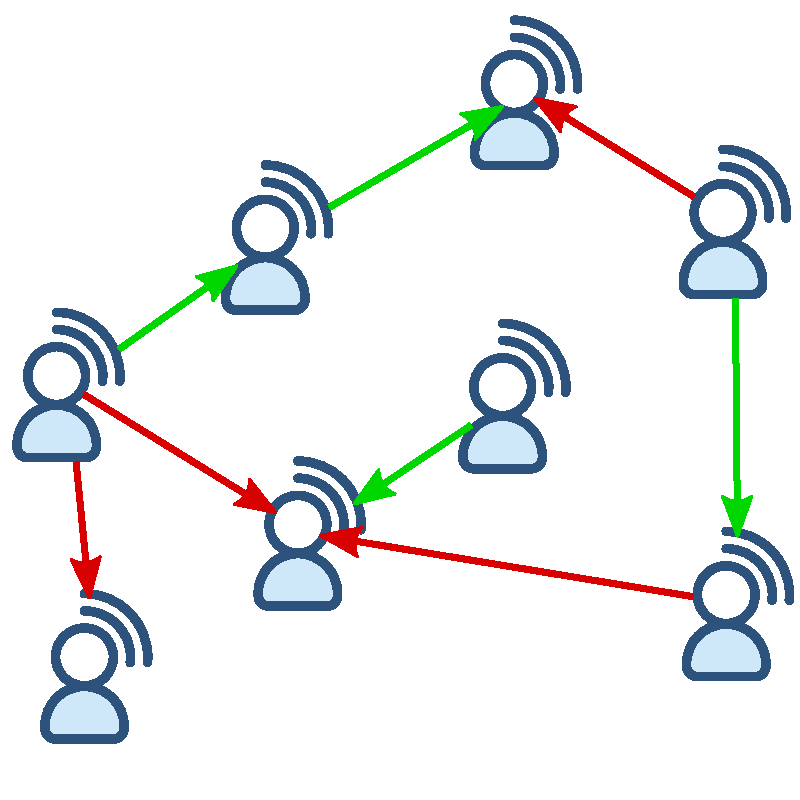
\includegraphics[height=6cm]{wiki.pdf}
  \end{center}
\end{frame}
\begin{frame}{More complex graphs -- Bipartite purchase}
  Bipartite purchase network: nodes are customers and products, edges
  are reviews

  \begin{center}
  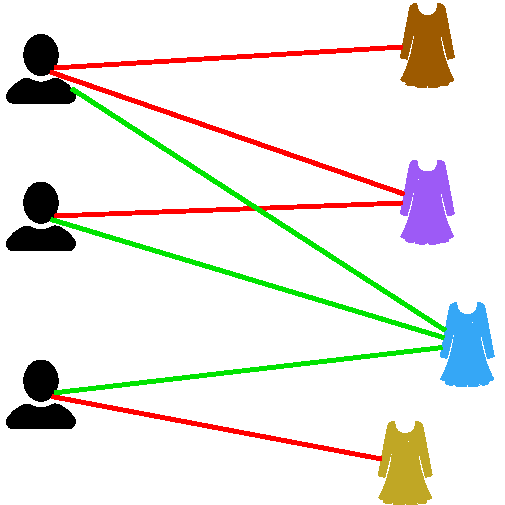
\includegraphics[height=7cm]{bipartite.pdf}
  \end{center}
\end{frame}
\begin{frame}{More complex graphs -- Co-purchase}
  Attributed co-purchase network: nodes are products and their
  characteristic, edges denotes “frequently purchased together”

  \begin{center}
  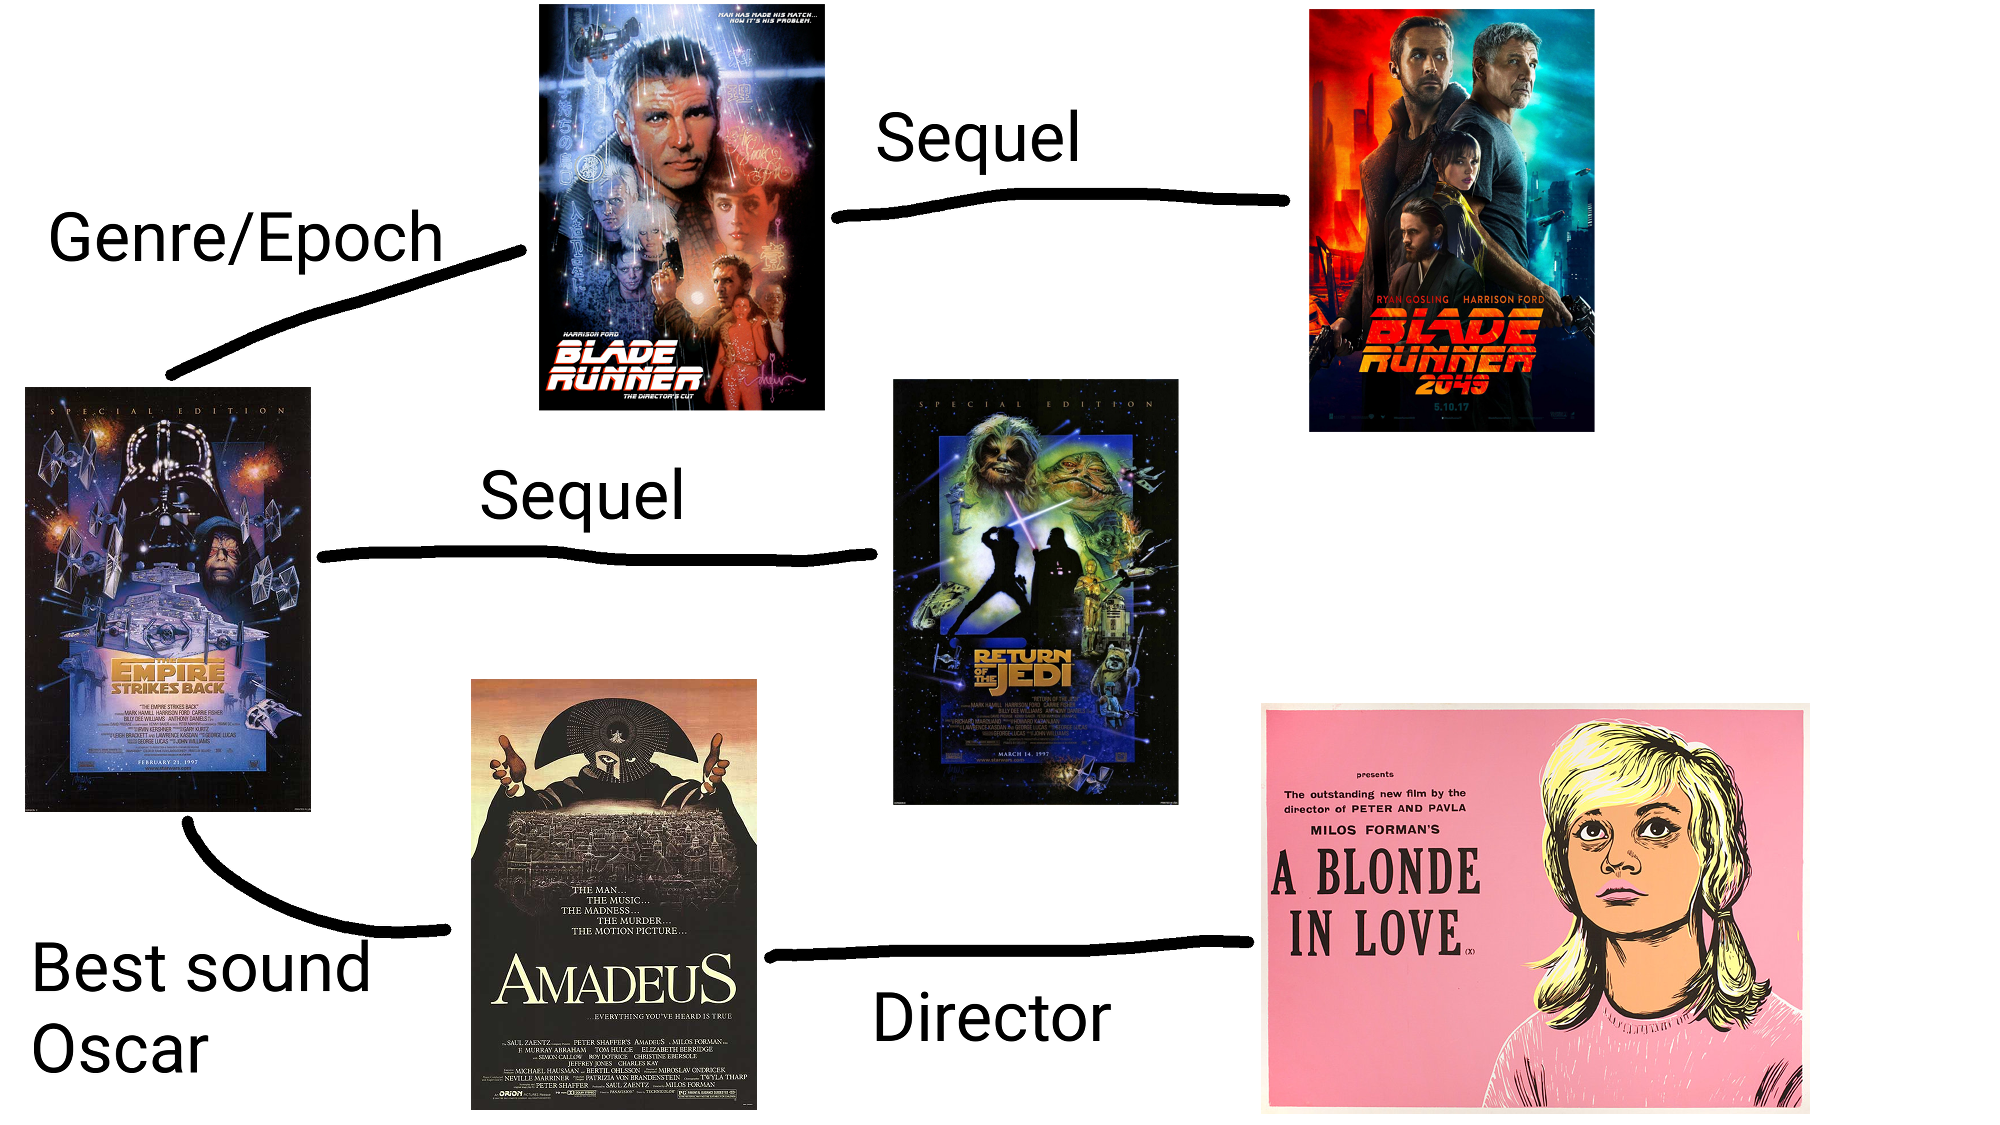
\includegraphics[height=8.5cm]{movies2.png}
  \end{center}
\end{frame}

\begin{frame}{Thesis statement}
\protect\hypertarget{thesis-statement}{}

\begin{itemize}
\item
  Such graphs are richer, but edge label might be costly to obtain,
  too numerous or missing.
\item
  Fortunately, I will show that \textbf{there exist \alert{efficient and accurate} methods to
  \alert{predict edge type} in \alert{complex networks}, relying only on the \alert{graph topology}
or also on \alert{node attributes}.}
\end{itemize}

\end{frame}

  \begin{frame}
    \frametitle{Outline}
    \tableofcontents%[currentsection]
  \end{frame}

\section{I - Directed signed graphs (8 mins)}
\label{i---directed-signed-graphs-8-minutes}

\begin{frame}{Motivations}

    More Directed signed social networks (DSSN) besides \wik{} editors:
\begin{description}
    \largelist
\item[\aut{}]
\(i\) cites the work of \(j\) to praise it or criticise it.

\item[\sla{}]
\(i\) considers \(j\) as a friend or foe.

\item[\epi{}]
\(i\) trusts or not the reviews made by \(j\).

\item[\kiw{}]
\(i\) reacted to a Wikipedia edit made by \(j\), to enhance it or revert it.
\end{description}

\end{frame}

\begin{frame}{Problem statement}

  Given the topology of a directed graph and the signs of some edges:
  predict the remaining signs \(\rightarrow\) batch binary
  classification

\begin{columns}[c]
\begin{column}{.55\textwidth}
    \includegraphics[height=5cm]{../assets/tikz/defense_signed_tikz.pdf}
\end{column}%
\hfill%
\begin{column}{.44\textwidth}
  Being able to predict edge signs let us solve \textbf{practical, real world problems}:
\end{column}%
\end{columns}
  % \begin{center}
  % \end{center}
  \begin{itemize}
    \tightlist
  \item
    ``Frenemy'' detection%;~\autocite{frenemy12};
  \item
    Automatic moderation of large scale online interactions
  \item
    Cyber bullying prevention, at school or in online games%~\autocite{CyberbullyingCHI15}.
\end{itemize}

\end{frame}

\begin{frame}{Solution Part 1: Generative model}
\protect\hypertarget{solution-part-1-generative-model}{}

The first ingredient is a sign generative model, made of 2 parameters $p$ and $q$
governing emitting and receiving behavior and drawn from a prior distribution $\mu$.

\begin{center}
\includegraphics{../assets/tikz/troll_genmodel_tikz.pdf}
\end{center}

\end{frame}

\begin{frame}{Solution Part 2: Graph transformation}
\protect\hypertarget{solution-part-2-graph-transformation}{}

The second one is a linear transformation of the graph, turning the
problem into node classification. Doing label propagation on that new
graph is an approximation of computing the maximum likelihood estimator
of \(p\) and \(q\).

\begin{columns}[c]
\begin{column}{.49\textwidth}
\includegraphics[height=5cm]{../assets/tikz/defense_original_tikz.pdf}
\end{column}%
\hfill%
\begin{column}{.49\textwidth}
\includegraphics[height=5cm]{../assets/tikz/defense_weighted_tikz.pdf}
\end{column}%
\end{columns}

\end{frame}

\begin{frame}{Solution Part 3: Theoretical guarantees}
\protect\hypertarget{solution-part-3-theoretical-guarantees}{}

Finally we show that when the graph is dense and the sampling uniform,
directly estimating \(p\) and \(q\) on training data has good
theoretical property, and performs well in practice anyway.

Namely, when we have $Q = \frac{1}{2\ve^2}\ln\frac{4|V|}{\delta}$ samples of outgoing and incoming
edges for every nodes, then, letting $\outqt{\htr}$, $\inqt{\hun}$ and $\biasqt{\tauhat}$ being
empirical estimates, we have that:

\begin{equation*}
\left|\Big[\outqt{\big(1-\htr_u\big)} + \inqt{\big(1-\hun_v\big)} -\biasqt{\tauhat} \Big] -
\Big[\frac{\outqt{p_u}+\inqt{q_v}}{2}\Big]\right| \leq 8\ve
\end{equation*}

\alert{holds with probability at least $1-10\delta$} simultaneously for all
non-queried edges $(u,v) \in E$ such that $\dout(u),\din(v) \ge Q$.

\end{frame}

\begin{frame}{Experiments: \epi{} dataset}
\protect\hypertarget{experiments-epinion-dataset}{}

\begin{table}[p]
  % \begin{adjustwidth}{-0.8cm}{}
    \small
  \centering
  \caption{$100\times$ MCC results on \epi{} as $|\Etrain|$ grows}
  \begin{tabular}{lcccccc|r}
    \toprule
    {}               & Global     & 3\%             & 9\%                & 15\%               & 20\%               & 25\%               & time (ms)     \\
    \midrule
    \uslogregp{}     &            & 43.51           & 54.85              & 59.29              & 61.45              & 62.95              & 32            \\
    \rowcolor{lightyellow}
    \usrule{}        &            & 41.39           & 53.23              & 57.76              & 60.06              & 61.93              & \textbf{7}    \\
    \rowcolor{lightyellow}
    \uslpropGsec{}   & \checkmark & \vsecond{51.47} & \vsecondSig{58.43} & \vsecondSig{61.41} & \vsecondSig{63.14} & \vsecondSig{64.47} & \textbf{1226} \\
    \midrule
    \compranknodes{} & \checkmark & \vfirst{52.04}  & \vfirstSig{60.21}  & \vfirstSig{62.69}  & \vfirstSig{64.13}  & \vfirstSig{65.22}  & \textbf{2341} \\
    \complowrank{}   & \checkmark & 36.84           & 43.95              & 48.61              & 51.43              & 54.51              & 121530        \\
    \compbayesian{}  &            & 31.00           & 48.24              & 56.88              & 61.49              & 64.45              & 116838        \\
    \comptriads{}    &            & 34.42           & 49.94              & 54.56              & 56.96              & 58.73              & 129           \\
    \bottomrule
  \end{tabular}
  % \end{adjustwidth}
\end{table}

\end{frame}

\begin{frame}{Experiments: \aut{} dataset}
\protect\hypertarget{experiments-citation-dataset}{}

\begin{table}[p]
  % \begin{adjustwidth}{-0.8cm}{}
  \centering
  \small
  \caption{$100\times$ MCC results on \aut{} as $|\Etrain|$ grows}
    \begin{tabular}{lcccccc|r}
    \toprule
    {}               & Global     & 3\%                & 9\%                & 15\%               & 20\%               & 25\%               & time (ms)            \\
    \midrule
    \uslogregp{}     &            & \vsecondSig{15.19} & \vsecondSig{26.46} & 32.98              & 36.57              & 39.90              & 2                    \\
    \rowcolor{lightyellow}
    \usrule{}        &            & 15.09              & 26.40              & \vsecondSig{32.98} & \vsecondSig{36.72} & 40.16              & \textbf{\textless 1} \\
    \rowcolor{lightyellow}
    \uslpropGsec{}   & \checkmark & \vfirstSig{19.00}  & \vfirstSig{30.25}  & \vfirstSig{35.73}  & \vfirstSig{38.53}  & \vfirstSig{41.32}  & \textbf{16}          \\
    \midrule
    \compranknodes{} & \checkmark & 12.28              & 24.44              & 31.03              & 34.57              & 38.26              & \textbf{128}         \\
    \complowrank{}   & \checkmark & 8.85               & 17.08              & 22.57              & 25.57              & 29.24              & 1894                 \\
    \compbayesian{}  &            & 10.91              & 23.75              & 32.25              & 36.52              & \vsecondSig{40.32} & 5398                 \\
    \comptriads{}    &            & 8.62               & 16.42              & 22.01              & 24.77              & 27.13              & 5                    \\
    \bottomrule
    \end{tabular}
  % \end{adjustwidth}
\end{table}

\end{frame}

\begin{frame}{Conclusion}
\protect\hypertarget{conclusion}{}

Because we only use the topology, our solution is both:

\begin{itemize}
\tightlist
\item
  domain agnostic
\item
  fast
\end{itemize}

\end{frame}

\section{II - Undirected signed graphs (8 minutes)}
\label{ii---undirected-signed-graphs-8-minutes}

\begin{frame}{Problem}

\begin{itemize}
\tightlist
\item
  Our sign generative model is not suitable for undirected graphs.\\
  Yet such graphs are important, for instance for recommendation in
  bipartite graphs.
\end{itemize}

\begin{columns}[T] % align columns
\begin{column}{.49\textwidth}
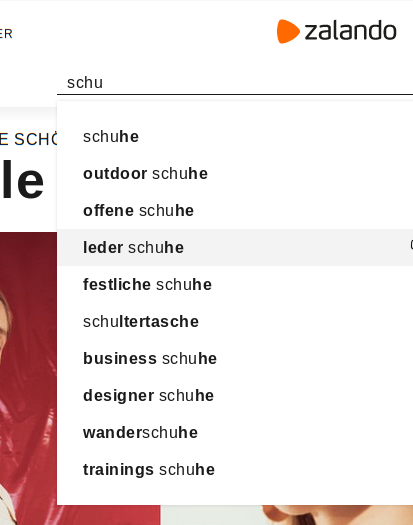
\includegraphics[height=5cm]{suggestions.png}
\end{column}%
\hfill%
\begin{column}{.49\textwidth}
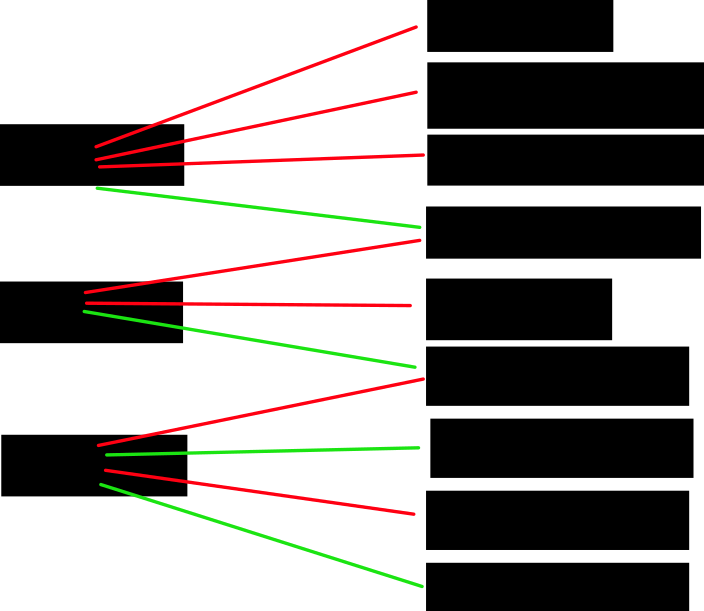
\includegraphics[height=5cm]{sugbipart.pdf}
\end{column}%
\end{columns}

\begin{itemize}
\tightlist
\item
  We consider the active setting, where we first select a training set,
  query its signs and predict the remaining edges.
\end{itemize}

\end{frame}

\begin{frame}{New bias}

\begin{itemize}
\item
  Assume that nodes belongs to \(K\) latent groups, and that signs are
  governed by those groups, modulo some irregularities.
  \begin{center}
  \includegraphics[height=3cm]{../assets/tikz/defense_kgroups_tikz.pdf}
  \end{center}
\item This is motivated in social networks by the balance theory and in other graphs by assortative/dissortative patterns.
\item
  Recovering those \(K\) groups in the presence of noise is the well
  studied Correlation Clustering problem (CC). The minimal objective
  value of CC when \(K=2\) is a bound on the number of mistakes for any
  active algorithms \autocite{Cesa-Bianchi2012b}.
\end{itemize}

\end{frame}

\begin{frame}{Solution: spanning structure}

\begin{itemize}
\item
  An interesting case is \(K\) = 2 (strong balance), if there was no
  noise, the sign of any edge would the parity of any path between its
  endpoint.
\item Since the noise is uniform (with probability $q$), the longer such path, the more likely we make an error by
  predicting using parity of observed edges. Overall, the expected number of errors is:
  \begin{equation*}
    q \left(|E| + \sum_{(u,v) \in E_{\mathrm{test}}} |\mathrm{path}^T(u, v)| \right)
  \end{equation*}
\item
  Thus we look for a spanning structure with few edges that aims to minimize the stretch.
\end{itemize}
\end{frame}

\begin{frame}{Construction}
  \begin{center}
    \includegraphics{../assets/tikz/gtx_eccentricity_tikz.pdf}
  \end{center}
\end{frame}

\begin{frame}{Experiments - Stretch}
\includegraphics{../assets/gtx_exp/gridst.pdf}
\end{frame}

\begin{frame}{Experiments - Stretch}
\includegraphics{../assets/gtx_exp/pasynthmcc.pdf}
\end{frame}


\section{III - Node attributed graphs (15 minutes)}
\label{iii---node-attributed-graphs-15-minutes}

\begin{frame}{Problem}
\protect\hypertarget{problem}{}

\begin{itemize}
\item
  Still characterizing edges, two big differences:

  \begin{itemize}
  \tightlist
  \item
    more than 2 types of edges \(\rightarrow\) \(k\)-multilayer graphs
  \item
    no label are provided at any point \(\rightarrow\) unsupervised
    problem
  \end{itemize}
\item
  Additional information: node \(u\) has a profile \(x_u \in [-1, 1]^d\)
\item
  Find \(k\) bounded “directions” and associate to every edge the “most
  explanatory” direction among those \(k\)
\end{itemize}

\end{frame}

\begin{frame}{Motivations}
\protect\hypertarget{motivations}{}

\begin{itemize}
\item
  BlaBlaCar: nodes are users described by experience, location,
  preferences (music, smoke, talk, pet), reviews, while edges are shared
  rides. Those rides could be to go to work, cultural events, vacations
  and so on.
\item
  Foursquare: nodes area venues described by location, reviews,
  category, time of visits, while edges are “frequently visited
  together” relation. Those venue groups can be part of party night,
  Sunday morning or sport routine.
\item
  We model nuanced relations driven both by partial homophily and
  heterophily.
\end{itemize}

\end{frame}

\begin{frame}{Formalization}
\protect\hypertarget{formalization}{}

\begin{itemize}
\item
  Combine the profiles of the
  \textcolor{DodgerBlue}{edge $u,v$ by entrywise product} and
  \textcolor{Orange}{score it} with
  \textcolor{Green}{direction $w_\ell$}:
\begin{equation*}
  \mathcolor{Orange}{\big(}\mathcolor{DodgerBlue}{x_u \circ x_v}\mathcolor{Orange}{\big)^T}
  \mathcolor{Green}{w_\ell}
\end{equation*}
\end{itemize}
\begin{columns}[T] % align columns
\begin{column}{.59\textwidth}
\begin{itemize}
\item
  Associate the \textcolor{HotPink}{"most explanatory" direction} to
  this edge:
  \begin{equation*}
    \mathcolor{HotPink}{\max_{\ell \in \{1, \ldots, k\}}} 
    \mathcolor{Orange}{\big(}\mathcolor{DodgerBlue}{x_u \circ x_v}\mathcolor{Orange}{\big)^T}
    \mathcolor{Green}{w_{\mathcolor{HotPink}{\ell}}}\quad\text{Let}\,
    \mathcolor{Green}{w_{\mathcolor{HotPink}{\ell}}} =
    \mathcolor{Green}{w(}\mathcolor{HotPink}{u,v}\mathcolor{Green}{)}
  \end{equation*}
\item
  Find the \textcolor{Teal}{overall best $k$ directions}:
  \begin{equation*}
    \mathcolor{Teal}{\argmax_{\{w_1,\ldots,w_k\} \subset \dball}
    \sum_{u,v \in E}}
    \mathcolor{HotPink}{\max_{\ell \in \{1, \ldots, k\}}} 
    \mathcolor{Orange}{\big(}\mathcolor{DodgerBlue}{x_u \circ x_v}\mathcolor{Orange}{\big)^T}
    \mathcolor{Green}{w_{\mathcolor{HotPink}{\ell}}}
  \end{equation*}
\end{itemize}
\end{column}%
\hfill%
\begin{column}{.42\textwidth}

{\small
  \setlength{\tabcolsep}{4pt}
  \begin{tabular}{rrrrrr}
    \toprule
    ${x_u}$ & ${x_v}$ & ${\mathcolor{DodgerBlue}{x_u \circ x_v}}$
            & $\mathcolor{Green}{w_1}$ & $\mathcolor{Green}{w_2}$ \\
    \midrule
    $0.9$  & $0.8$  & $0.72$  & $0.6$  & $0.1$ \\
    $-0.8$ & $-0.9$ & $0.72$  & $0.1$  & $0.4$ \\
    $0.9$  & $-0.8$ & $-0.72$ & $-0.7$ & $0.6$ \\
    $0.0$  & $0.5$  & $0.0$   & $0.1$  & $0.4$ \\
    \bottomrule
  \end{tabular}
}

$\mathcolor{Orange}{\big(}\mathcolor{DodgerBlue}{x_u \circ x_v}\mathcolor{Orange}{\big)^T} \mathcolor{Green}{w_1} = 1.008$
$\mathcolor{Orange}{\big(}\mathcolor{DodgerBlue}{x_u \circ x_v}\mathcolor{Orange}{\big)^T} \mathcolor{Green}{w_2} = -0.072$
\end{column}%
\end{columns}

\end{frame}

\begin{frame}{Two Topological Constraints}
\protect\hypertarget{two-topological-constraints}{}

\begin{enumerate}
  \item The profile of each node is (close to) a linear combination of its incident directions: this
    introduces additional parameters ($\{a_{uv}\}_{u,v \in E}$ and $\{b_u\}_{u \in V}$) but provides more guidance.

\begin{equation*}
  \mathcal{L}_{\mathrm{node}} =
  \sum_{u\in V} \left|\left| x_u - b_u -
  \sum_{v \in \mathcal{N}(u)} a_{uv} 
    \mathcolor{Green}{w(}\mathcolor{HotPink}{u,v}\mathcolor{Green}{)}
 \right|\right|^2_2
\end{equation*}

  \item Each node can only be involved in \(k_\mathrm{local} < k\) directions.

\begin{equation*}
  \label{eq:edge_local_loss}
  \mathcal{L}_{\mathrm{local}} =
  \sum_{u \in V} \left\| \sum_{v \in \nei(u)} y_{uv} \right\|_1
  % = \sum_{u \in V} \left( \sum_{i = 1}^k \sum_{v \in \nei(u)}
  % \frac{\exp(\beta g(s_{uv}, w_i))}{\sum_{j=1}^k \exp(\beta g(s_{uv}, w_j))} \right)
\end{equation*}
Think of $y_{uv}$ as an indicator vector with $k$ components. Its $i^{th}$ component can be relaxed
to

\begin{equation*}
  {y_{uv}}_{;i} = \frac{\mathcolor{Sienna}{\exp(\beta} 
    \mathcolor{Orange}{\big(}\mathcolor{DodgerBlue}{x_u \circ x_v}\mathcolor{Orange}{\big)^T}\mathcolor{Green}{w_i}
  \mathcolor{Sienna}{)}}%
  {\mathcolor{Sienna}{\sum_{j=1}^k \exp(\beta} 
    \mathcolor{Orange}{\big(}\mathcolor{DodgerBlue}{x_u \circ x_v}\mathcolor{Orange}{\big)^T}\mathcolor{Green}{w_j}
  \mathcolor{Sienna}{)}}
\end{equation*}
\end{enumerate}

\end{frame}

\begin{frame}{First Solutions}
\protect\hypertarget{first-solutions}{}

\begin{itemize}
\item
  A baseline is simply to cluster the \(|E| \, \mathcolor{DodgerBlue}{x_u \circ x_v}\) in \(k\)
  clusters.
\item
  It can be improved by plugging our scoring function in the Lloyd
  algorithm.
\item
  Another approach is to directly optimize our objective function. We first make it convex by
  \textcolor{Sienna}{relaxing \(\mathcolor{HotPink}{\max}\) using softmax}.

  \begin{equation*}
    \mathcolor{Teal}{\argmax_{\{w_1,\ldots,w_k\} \subset \dball}
    \sum_{u,v \in E}}
    \mathcolor{Sienna}{\frac{1}{\beta}}
    \mathcolor{Sienna}{\sum_{\ell=1}^k\log\Big(\exp\big(\beta}
        \mathcolor{Orange}{\big(}\mathcolor{DodgerBlue}{x_u \circ x_v}\mathcolor{Orange}{\big)^T}
        \mathcolor{Green}{w_{\mathcolor{Sienna}{\ell}}}
    \mathcolor{Sienna}{\big)\Big)}
  \end{equation*}
Then we take topology into account, by relaxing as well the two previous
  regularization terms, and optimize the difference of convex terms by gradient
  descent\footnote{Disciplined Convex-Concave Programming}
\end{itemize}

\end{frame}

\begin{frame}{Matrix Solution -- Convex formulation}
\protect\hypertarget{matrix-solutions}{}

\begin{itemize}
\item
  Find a direction for each edge, but make sure those directions are
  linear combination of \(k\) “base” directions \(\rightarrow\) \textcolor{Peru}{low rank
  matrix}.

  \begin{equation*}
    \sum_{u,v \in E}
    \mathcolor{Orange}{\big(}\mathcolor{DodgerBlue}{x_u \circ x_v}\mathcolor{Orange}{\big)^T}
    \mathcolor{Green}{w_{uv}}
    = \mathcolor{Orange}{\big\langle} \mathcolor{DodgerBlue}{S^T} \mathcolor{Orange}{,}
    \mathcolor{Green}{W} \mathcolor{Orange}{\big\rangle_\mathrm{F}}
  \end{equation*}

  \begin{equation*}
    \mathcolor{Teal}{\min_{W\in \mathbb{M}^{d\times |E|}}}
    -\mathcolor{Orange}{\big\langle} \mathcolor{DodgerBlue}{S^T} \mathcolor{Orange}{,}
    \mathcolor{Green}{W} \mathcolor{Orange}{\big\rangle_\mathrm{F}} + \mathcolor{Peru}{\rank(W)}
  \end{equation*}

\item
  Relax low rank by \textcolor{Peru}{nuclear norm} and ensure \textcolor{Peru}{the norm of \(W\)
  columns are not too large}. Optimized by the Frank Wolfe method, only requiring top singular
  vector at each iteration.

  \begin{equation*}
    \mathcolor{Teal}{\min_{\substack{W\in \Rbb^{d\times |E|} \\ \mathcolor{Peru}{\|W\|_* \leq \delta}}}}
    \mathcolor{Orange}{\big\langle} \mathcolor{Peru}{\mu W}
      -\mathcolor{DodgerBlue}{S^T} \mathcolor{Orange}{,}
    \mathcolor{Green}{W} \mathcolor{Orange}{\big\rangle_\mathrm{F}}
  \end{equation*}
\end{itemize}
\end{frame}

\begin{frame}{Matrix Solution -- Alternating formulation}
\begin{itemize}
\item
  Write \(W\) explicitly as \(PQ^T\) and use alternating optimization.
\item
  Those formulations have more parameters, but allow mixed membership.
\end{itemize}

\end{frame}

\begin{frame}{Synthetic experiments}
\protect\hypertarget{synthetic-experiments}{}

% \begin{itemize}
% \tightlist
% \item
% \end{itemize}
  we generate data in order to have ground truth: (500 nodes, 1300 edges, 200 times $k$ directions
  and corresponding profiles)

% \begin{adjustwidth}{-.5cm}{}
  % \small
  \begin{tabulary}{\textwidth}{llll|ll}
    \toprule
    \thead{$\mathcal{D}_k$} & \thead{\kmeans{}} & \thead{\lloyd{}}                      &
    \thead{\combined{}}                  & \thead{\textsc{Frank Wolfe}} & \thead{\pqt{}} \\
    \midrule
    {\default{}}            & $.818 $           & $\esecondSig{.873 }\spval{1.25}{-63}$ & $\efirstSig{.893 }\spval{5.68}{-33}$ & $.381 $                      & $.893 $        \\
    {\smallk{}}             & $.836 $           & $\esecond{.838 }$                     & $\efirstSig{.875 }\spval{2.17}{-58}$ & $.213 $                      & $.875 $        \\
    {\largek{}}             & $.803 $           & $\esecondSig{.881 }\spval{2.66}{-94}$ & $\efirstSig{.894 }\spval{8.98}{-17}$ & $.421 $                      & $.894 $        \\
    {\smallo{}}             & $.813 $           & $\esecondSig{.824 }\spval{7.57}{-6}$  & $\efirstSig{.856 }\spval{2.99}{-57}$ & $.378 $                      & $.855 $        \\
    {\largeo{}}             & $\esecond{.827 }$ & $.823 $                               & $\efirstSig{.852 }\spval{1.90}{-25}$ & $.370 $                      & $.851 $        \\
    {\fdirs{}}              & $.772 $           & $\esecondSig{.814 }\spval{6.02}{-42}$ & $\efirstSig{.853 }\spval{2.13}{-47}$ & $.320 $                      & $.853 $        \\
    {\larged{}}             & $.905 $           & $\esecondSig{.933 }\spval{1.32}{-31}$ & $\efirstSig{.941 }\spval{1.77}{-22}$ & $.222 $                      & $.931 $        \\
    \bottomrule
  \end{tabulary}
% \end{adjustwidth}

\end{frame}


\begin{frame}{Conclusions}

\begin{itemize}
    \item
      Given a graph with node profiles, find $k$ directions explaining the existing connections
    \item
      linear model for performance and interpretability, two formulations:
    \begin{itemize}
      \item difference of convex scalar functions
      \item Matrix convex expression suitable for Frank--Wolfe algorithm
    \end{itemize}
    \item
      Future work:
    \begin{itemize}
      \item take time into account (homophily vs contagion)
      \item multigraph, more than one type of edge between two nodes
    \end{itemize}
\end{itemize}

\end{frame}

\section{IV - Conclusion (6 minutes)}
\label{iv---conclusion-6-minutes}

\begin{frame}{Contribution}
\protect\hypertarget{contribution}{}

\textbf{efficient and accurate methods to predict edge type in complex
networks, relying only on the graph topology or also on node
attributes.}

\begin{adjustwidth}{-.31cm}{}
  \small
  \setlength{\tabcolsep}{4pt}
  \begin{tabulary}{0.9\paperwidth}{lLLL}
    \toprule
    & I & II & III \\
    \midrule
    graph            & directed, 2 types      & undirected, 2 types           & attributed, $k$ types \\
    learning setting & batch label            & active label                  & no label \\
    approach         & estimate parameters    & find spanning structure       & matrix optimization \\
    efficient        & $O(|E|)$, parallel & $O(|E|\log |E|)$, conjectured & $O(dT|E|)$ \\
    accurate &
    close to Bayes predictor, efficient in practice &
    Close to Correlation Clustering bound &
    convex problem: global max (but no ground truth) \\
    \bottomrule
  \end{tabulary}
\end{adjustwidth}

\end{frame}

\begin{frame}{Future work}
\protect\hypertarget{future-work}{}

\begin{itemize}
\tightlist
\item
  Two ways relation with representation learning in graphs:

  \begin{itemize}
  \tightlist
  \item
    can give more accurate input to RL methods
  \item
    can exploit RL features as node attributes
  \end{itemize}
\item
  \emph{link prediction as Liva suggested?}
\end{itemize}

\end{frame}

\begin{frame}{References}
  \printbibliography
\end{frame}

\begin{frame}[plain,c]

\begin{center}
\Huge Thank you! \\ Questions?
\end{center}

\end{frame}

\appendix


\begin{frame}{Setting}

The signs are \textbf{adversarial} rather than generated by our model.

At each round, the learner is asked to predict one label, which is then revealed to him and the
procedure repeats.

\end{frame}

\begin{frame}{Labeling regularity}

% Inspired by trollness and trustworthiness, we define the regularity of a labeling \(Y\).

Letting $Y$ be the vector of all labels, $\Psiout(i, Y)$ is the number of least used label outgoing
from $i$, and $\Psiout(Y) = \sum_{i \in V} \Psiout(i,Y)$.

Likewise for incoming edges, \(\Psiin(Y) = \sum_{j \in V} \Psiin(j,Y)\) and finally
\(\Psi_G(Y) = \min\big\{\Psiin(Y), \Psiout(Y)\big\}\).

% This can be read from the cutsize of \(G'\)
\begin{columns}[T]
  \begin{column}{0.6\textwidth}
    % \vspace{-2cm}
    \begin{tabular}{lcccc|l}
      \toprule
      node $i$        & $1$ & $2$ & $3$ & $4$ &                  \\
      \midrule
      $\Psiout(i, Y)$ & 0   & 0   & 1   & 0   & $\Psiout(Y) = 1$  \\
      $\Psiin(i, Y)$  & 1   & 0   & 0   & 1   & $\Psiin(Y) = 2$ \\
      \bottomrule
    \end{tabular}
  \end{column}%
  \hfill%
  \begin{column}{0.39\textwidth}
    \centering 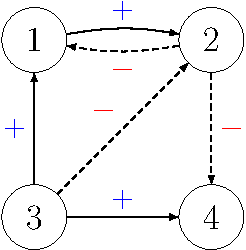
\includegraphics[height=.35\textheight]{../assets/raw/g_latex-crop}
  \end{column}%
\end{columns}

\end{frame}

\begin{frame}{Online algorithm and bounds}
  \begin{itemize}[<+->]
    \largelist
  \item 
    Our algorithm is a combination of Randomized Weighted Majority instances built on top of each other. 

  \item 
    On average, it makes $\Psi_G(Y) + O\left(\sqrt{|V|\Psi_G(Y)} + |V|\right)$ mistakes.

  \item 
    On the lower side,
    % Up to this $O\left(\sqrt{|V|\Psi_G(Y)} + |V|\right)$ factor, it is optimal as we can show that 
    for any directed graph $G$ and any integer $K$,
    there exists a labeling $Y$ forcing at least $\frac{K}{2}$ mistakes to any online algorithms,
    while $\Psi_G(Y) \leq K$.
\end{itemize}

\end{frame}

\begin{frame}{Online algorithm, 1. RWM node instances}

For each node \(i\), we predict the sign of edge outgoing from \(i\) by
relying on two constant experts, always predicting \(-1\) or always
predicting \(+1\). The best one will make \(\Psiout(i, Y)\) mistakes. We
combine them in a Randomized Weighted Majority algorithm (RWM) instance
associated with \(i\), call it \(RWM_{out}(i)\). The instance expected
number of mistakes is therefore~\autocite{acg02},
denoting by \(M(i,j)\) the indicator function of a mistake on edge
\((i,j)\)
\[\sum_{j \in \Nout(i)} \E\,M(i,j) = \Psiout(i,Y) + O\left(\sqrt{\Psiout(i,Y)}+ 1\right)\]

We use the same technique to predict incoming edges of each node \(j\),
the instance \(RWM_{in}(j)\) having the following average number of
mistakes
\[\sum_{i \in \Nin(j)} \E\,M(i,j) = \Psiin(j,Y) + O\left(\sqrt{\Psiin(j,Y)} + 1\right)\]

\end{frame}

\begin{frame}{Online algorithm, 2. combining instances}

We then define two meta experts: \(RWM_{out}\), which predicts
\(y_{i,j}\) as \(RWM_{out}(i)\), and \(RWM_{in}\), which predicts
\(y_{i,j}\) as \(RWM_{in}(j)\). Summing over all nodes, the number of
mistakes of these two experts satisfy

\begin{align*}
    \sum_{i \in V}\sum_{j \in \Nout(i)} \E\,M(i,j) &= \Psiout(Y) + O\left(\sqrt{|V|\Psiout(Y)} + |V|\right) \\
    \sum_{j \in V}\sum_{i \in \Nin(j)} \E\,M(i,j)  &= \Psiin(Y)  + O\left(\sqrt{|V|\Psiin(Y)}  + |V|\right)
\end{align*}
\end{frame}

\begin{frame}{Online algorithm, 3. final prediction}

Our final predictor is a RWM combination of \(RWM_{out}\) and
\(RWM_{out}\), whose expected number of mistakes is
\begin{alignat*}{3}
    \sum_{(i,j) \in E} \E\,M(i,j) 
    &= \Psi_G(Y) + O\Biggl(&&\sqrt{|V|\Psi_G(Y)} + |V| \\
  & &&+ \sqrt{\Bigl(\Psi_G(Y) + |V| + \sqrt{|V|\Psi_G(Y)}\Bigr)} \Biggr)\\
    &= \Psi_G(Y) + O\Bigl( &&\sqrt{|V|\Psi_G(Y)} + |V|\Bigr)
\end{alignat*}

\end{frame}

\begin{frame}{Datasets properties}

\begin{table}
  \centering
  % \small
  \caption{Dataset properties. \label{tab:dataset}}
  \begin{tabular}{lrrrrrrrr}
    \toprule
    Dataset & $|V|$       & $|E|$       & $\frac{|E|}{|V|}$ & $\frac{|E^+|}{|E|}$ & $\frac{\Psi_{G''}(Y)}{|E|}$ & $\frac{\Psi_G(Y)}{|E|}$ \\
    \midrule
    \aut{}  & \np{4831}   & \np{39452}  & 8.1               & 72.33\%             & .076                        & .191                    \\
    \wik{}  & \np{7114}   & \np{103108} & 14.5              & 78.79\%             & .063                        & .142                    \\
    \sla{}  & \np{82140}  & \np{549202} & 6.7               & 77.40\%             & .059                        & .143                    \\
    \epi{}  & \np{131580} & \np{840799} & 6.4               & 85.29\%             & .031                        & .074                    \\
    \kiw{}  & \np{138587} & \np{740106} & 5.3               & 87.89\%             & .034                        & .086                    \\
    \bottomrule
  \end{tabular}
\end{table}

$$\Psi_{G''}(Y) = 
\min_{\bp,\bq\in[0,1]^{|V|}}
\sum_{(i,j) \in E} \left(\frac{1+y_{i,j}}{2} - \frac{p_i+q_j}{2}\right)^2$$

\end{frame}

\begin{frame}{Data generation}
\protect\hypertarget{data-generation}{}

\begin{itemize}
\item
  create a random graph and pick for each a set of \(k_\mathrm{local}\)
  directions.
\item
  pick for each edge \((u,v)\) a direction index \(y_{uv} \in \rangesk\)
  among the ones shared by its endpoint.
\item
  draw the \(k\) directions at random
\item
  optimize the profiles so as to maximize the edges goodness, minimize
  the term \(\mathcal{L}_{\mathrm{node}}\) and enforces as much as
  possible that for every edge \((u,v) \in E\),
  \(\mathcal{E}(u,v) = y_{uv}\).
\end{itemize}

\emph{(take a look a Liva comment about Lagrangian relaxation of integer
program\ldots{})}

\end{frame}
\end{document}
